\documentclass{article}

\usepackage[final]{nips_2016}

\usepackage[utf8]{inputenc} % allow utf-8 input
\usepackage[T1]{fontenc}    % use 8-bit T1 fonts
\usepackage{hyperref}       % hyperlinks
\usepackage{url}            % simple URL typesetting
\usepackage{booktabs}       % professional-quality tables
\usepackage{amsfonts}       % blackboard math symbols
\usepackage{nicefrac}       % compact symbols for 1/2, etc.
\usepackage{microtype}      % microtypography
\usepackage{graphicx}
\usepackage{makecell}
\usepackage{algorithm}% http://ctan.org/pkg/algorithms
\usepackage{algpseudocode}%
\usepackage{bm}
\usepackage{amsmath}
\usepackage{makecell}
\usepackage{titlesec}

\title{The Effect of Noise on Hemorrhage Detection using CT Scan Imaging}

\author{%
  Joao Cardoso \\
  Institute for Enterprise Engineering (Artificial Intelligence)\\
  Duke University, Durham, NC 27708\\
  \texttt{joao.cardoso@duke.edu} \\
  % examples of more authors
   \And
Pushti Desai \\
Department of Biomedical Engineering \\
Duke University, Durham, NC 27708 \\
 \texttt{pushti.desai@duke.edu} \\
   \AND
Jasmine King \\
Department of Mechanical Engineering \\
Duke University, Durham, NC 27708 \\
 \texttt{jak110@duke.edu} \\
  \AND
Preethi Krishnan \\
Department of Biomedical Engineering \\
Duke University, Durham, NC 27708 \\
 \texttt{preethi.krishnan@duke.edu} \\
}

\begin{document}

\maketitle

\begin{abstract}
  CT images are affected by multiple physical  like sensor noise, temperature (thermal/Johnson-Nyquist noise), electrical charges, background radiation, and photon counting. In this study, we simulate CT noise by applying Gaussian and Poisson noise to the sinogram of CT Scans and utilize the reconstructed images to detect Intracranial Hemorrhage (ICH) using the publicly available RSNA dataset. Our results show that a physics-informed VGG pipeline can perform effectively with simulated noise. 
\end{abstract}

\section{Introduction}
\begin{par}
    Computed Tomography (CT) also known as computed axial tomography (CAT or CT scan) is a widespread imaging modality widely used in hospitals for medical diagnosis. Digital geometry processing is used to generate a three-dimensional image of an organ using two-dimensional X-ray images taken around a single axis of rotation [1]. The internal structure of the organ including fine details, dimensions, shape, internal defects, and density are reproduced in the CT image with speed and clarity. The CT mechanism involves an X-ray source that transmits X-rays on to the patient from various angles and the reflected data is transformed to digital signals. This raw data can be represented in the form of the image which is known as Sinogram and is computed using the radon transform. Inverse Radon transform is performed over the Sinogram to obtain the reconstructed CT image [2].
\end{par}

\begin{par}
    Intracranial hemorrhage (ICH) is a life threatening emergency and is defined as any bleeding within the intracranial vault, including the brain's parenchyma and surrounding meningeal spaces [3]. 
    Early diagnosis of ICH is important because of the rapid progression of neurological deterioration and cardiopulmonary instability [4]. Neuroimaging using CT scan is a critical tool for early diagnosis of ICH [5]. The drawbacks of using CT for head pathology are the radiation burden, lowered contrast, and the inclusion of artifacts and noise. The X rays ionizing effects may put patients at risk for increased radiation exposure. To prevent the harmful effects of radiation CT denoising algorithms were developed. The denoising techniques help in the reduction of radiation doses and also improve the overall  quality of images obtained from low-dose CT scans [6]. Increase in the radiation dose can lead to reduction in the noise level in CT images and improves resolution and image clarity. However, this leads to increase radiation exposure for the patient [7]. Therefore it is  important to achieve a balance between reducing radiation dose, implementation of efficient denoising techniques to improve image quality.
\end{par}

\begin{par}
    Our objective of this study is to develop a novel physics informed CNN model that can effectively detect intercranial haemorrhage. In this study, we simulate CT noise for a real-world dataset and experiment to find the optimal noise threshold that does not affect overall performance. To compare the diagnostic performance we compare different kinds of noise and show associated metrics for each noise. 
\end{par}

\section{Related Work}

\subsection{CT Noise Reduction Algorithms}

\begin{par}
    The major factors affecting the quality of reconstructed CT images are blurring due to patient movement, field of view abnormalities, artifacts due to beam hardening, software/hardware artifacts, and noise due to acquisition and transmission [2]. The balance between image quality and low radiation is paramount when diagnosis are made using CT technology [8]. The major sources of noise affecting CT images are random noise, statistical noise, electronic noise and round-off errors. Random and statistical noise are caused due to fluctuations due to the X ray quanta. Electrical noise is caused due to the analog electrical circuits.Round off errors are caused due to the quantization process during analog to digital conversion [2].
\end{par}

\begin{par}
    Traditional denoising methods used widely in CT noise reduction includes projection based techniques using radon transformation, wavelet transform, filtering, and dictionary methods. Filtered back propagation is used on sinogram through radon trasnsfromation to suppress noise in CT images. However, projection based iterative methods are computationally expensive [9]. Wavelet-based method uses the discrete complex wavelet transform and laplacian probability density functions are used to remove the noise in the transform domain [10]. However wavelet based methods do not perform efficiently for higher dimensional data due to poor directional sparsity [11]. A combination   model of  Wiener filtering and edge detection method has shown reduction in CT noise by modifying the kernel size and  threshold values in the edge detection [12].
    Dictionary denoising algorithm uses high spatial correlation between between images obtained from high and low energy spectra. The improvement in signal-to-noise ratio is due to a weighing addition function that uses normalized patches while reducing noise [13]. 
\end{par}

\begin{par}
    Deep learning methods have revolutionized CT image denoising and have been widely used to improve image resolution, and are computationally efficient with better performance compared to traditional methods [14]. CNN uses convolutional filters to extract features from the noisy input images using non linear transformation and produce denoised output images [15]. Advantages of CNN include handling high dimensional data, automatic feature extraction, and faster computational speed. The disadvantages of CNN are that a large number of annotated scans are required for the CNN to perform effectively and the model is a  black box without any interpretability [16]. Generative Adversarial Networks (GAN) use a generator and discriminator network to produce real CT images from noisy scans. The advantages of GAN are the generated images are realistic and are far superior in preserving intricate patterns compared to traditional denoising approaches. However, GANs have many disadvantages such as being computationally expensive, and inaccurate predictions that are clinically inaccurate [17]. CycleGAN and WGAN have been used for CT denoising as they can be trained on unpaired data and helps in preserving image details [18]. The  transformer can process each part of the CT image separately and can detect spatial dependencies among non linear segments. It detects important patterns in multiple regions of interest and is able to separate noise. In comparison to CNN, transformers can handle large images easily [19]. The disadvantages of using a transformer model is that the self-attention mechanism can sometimes choose noisy features and ignore important features in the CT scan [20]. 
\end{par}

\subsection{Dataset}

\begin{par}
    The Radiological Society of North America (RSNA) is a multi-institutional, and multinational brain hemorrhage CT dataset. It is one of the largest public real world dataset datasets with expert clinical annotations from multiple radiologists for subarachnoid, intraventricular, subdural, epidural, or intraparenchymal hemorrhages [21]. This dataset has a representation of a large variety of cerebral pathologic states and is ideal for machine learning applications. As a multinational dataset it has patients from different races and can help in reducing bias in machine learning algorithms.
\end{par}

\section{Methods}

In Figure 1, it is possible to see an overview of the data was generated, split in training and testing, passes through a denoising layer, and finally passed through the CNN to get a binary classification for presence of ICH.

\begin{figure}[h]
    \centering
    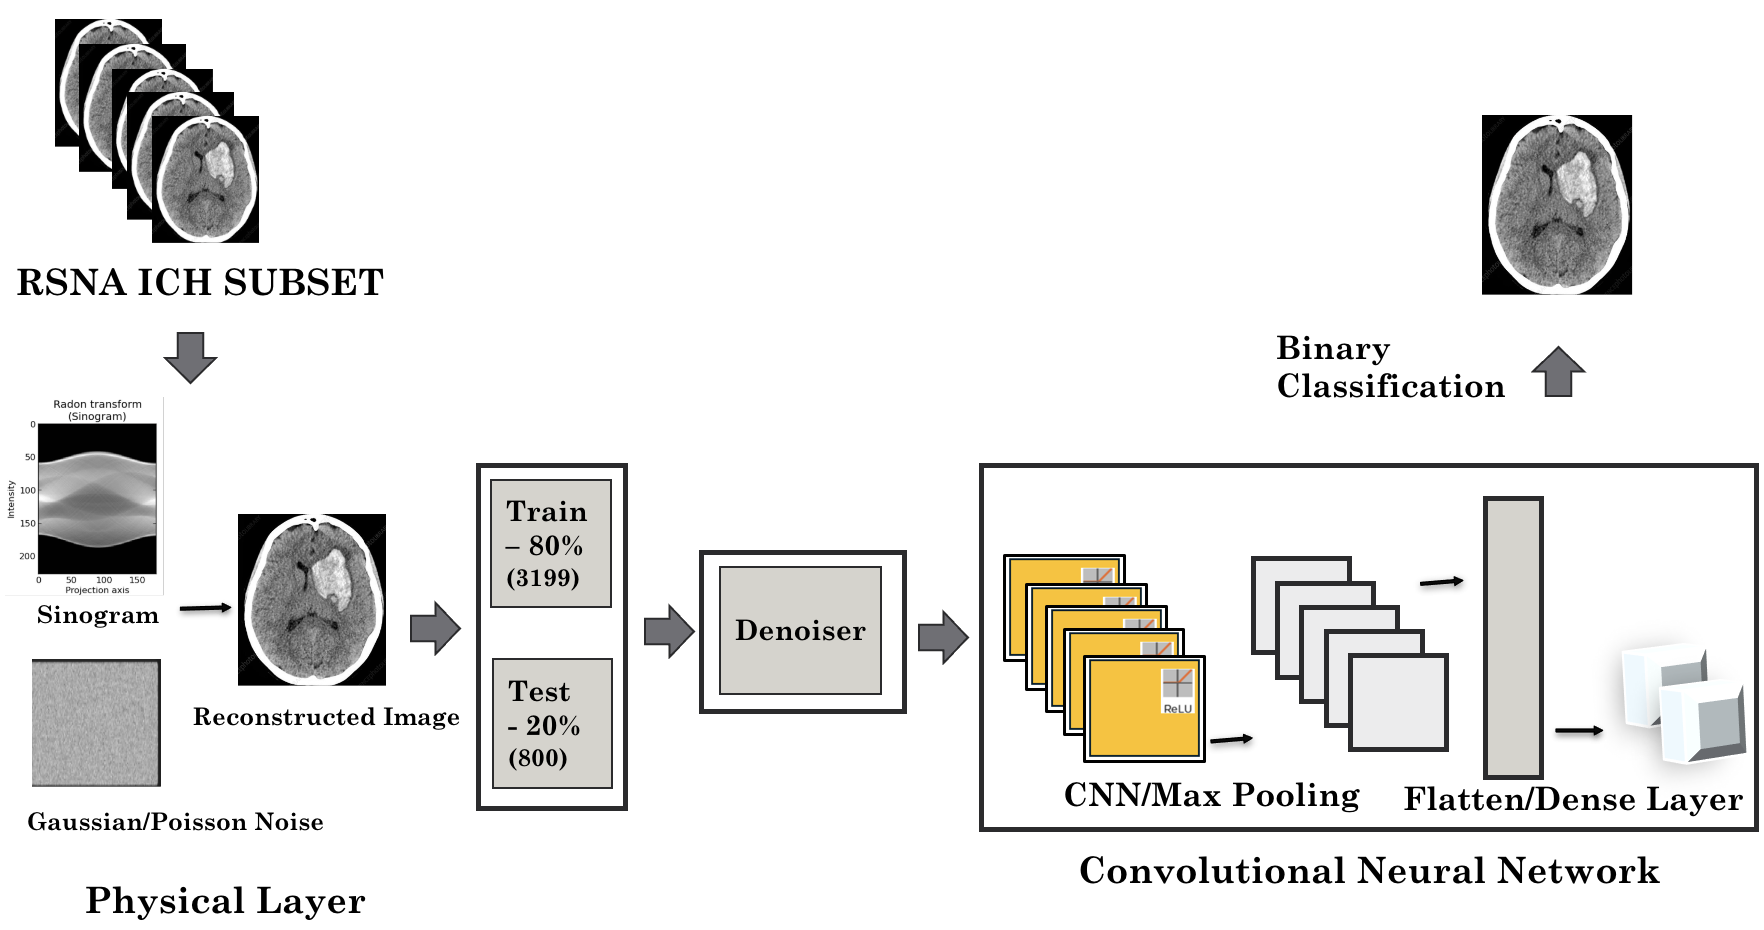
\includegraphics[width=1\textwidth]{pipeline.png}
    \caption{Solution Pipeline} 
\end{figure}

\subsection{Data Processing}
\begin{par}
    Based on a subset of 4000 samples from the RSNA ICH dataset, we initially converted the DICOM files to PNG using the DICOM Converter executable tool for MacOS. Then we implemented a pipeline to generate a train test split, and then produce new copies of those samples for each noise level to be used during both training and validation.
\end{par}

\subsection{Model}

\begin{par}
    We designed a deep convolution neural network that allows for the binary classification of images with and without hemorrhages. The model is based on VGG16 and is structured as a series of convolution blocks that takes the input image followed by a classification head. Each convolution block consists of the specified number of repetitions of a convolution layer with the same number of filters as inputted and kernel size of 3x3. Then, these convolution layers are followed by a max pooling layer with a 2x2 pool size and a stride of 2 in each block. These convolution blocks serve as a complex feature extraction from the input images, and finally, these features are inputted into the classification head to make the final decision.
    
    Here is a breakdown of our model's architecture:
    \begin{enumerate}
    \item Convolution Blocks: These blocks are structured with the number of filters increasing with each block to capture more and more refined features. The same padding is used for all convolution layers to make sure that the output feature maps have the same spatial dimensions as the input. Max pooling is applied after convolution layers in each block to reduce the feature map dimensions so that the computational load and number of parameters is decreased, preventing overfitting.

    \item Classification Head: The classification head takes the features from the convolution blocks and performs a binary classification with 1 representing a hemorrhage being present in the input image and 0 representing no hemorrhage is present in the input image.
    \end{enumerate}
\end{par}

\subsection{Physical Transformations}

\subsubsection{Addition of Noise}

\begin{par}
    Noise is added through a process where an image is transformed into its sinogram representation using Radon transform, noise is added, and then the sinogram is reconstructed back into an image using inverse Radon transform. Here is a detailed breakdown of the function and its components' functionalities:
    \begin{enumerate}
    \item Sinogram Transformation:
    A sinogram is created by projecting the image using Radon Transform. This Radon Transform calculates the projection at different angles and the number of angles is determined by dividing the maximum dimension of the input image by 8. This division creates a sub-sampling factor of 8 to reduce the computational cost while also maintaining the quality of the sinogram.
    
    \begin{figure}[h]
        \centering
        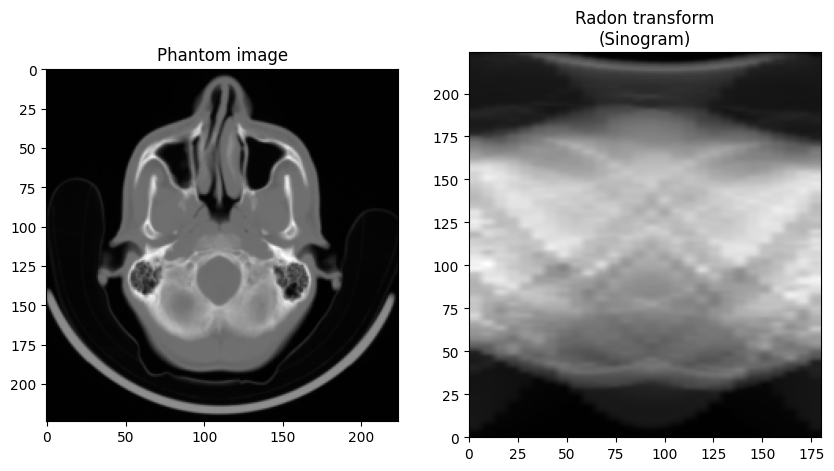
\includegraphics[width=0.5\textwidth]{sinogram.png}
        \caption{Sinogram generation via radon transform} 
    \end{figure}
    
    \item Noise Addition:
    Noise is simulated in these sinogram projections based on the inputted noise level. If a noise\_level of 0 is inputted, no noise is added and the image is directly reconstructed. If a non-zero noise\_level is inputted, Gaussian noise is added using the random\_noise function from skimage.util. The variance of Gaussian distribution is set by squaring the noise\_level so that a higher noise\_level results in noise with a wider spread of values, affecting the noise more significantly. Clipping is also turned off to allow for pixel values to exceed the bounds of 0 to 255.
    
    \item Image Reconstruction:
    The sinogram is reconstructed into an image used inverse Radon transform using a ramp filter. This filter increases the quality of the reconstructed image by compensating for the loss of low-frequency signals in the inverse Radon transform.
    
    \begin{figure}[h]
        \centering
        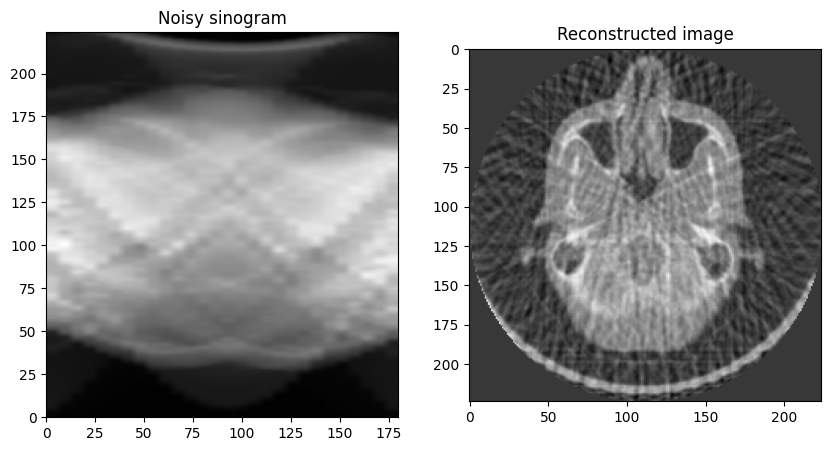
\includegraphics[width=0.5\textwidth]{sinogram_noise.png}
        \caption{Sinogram after applying noise and reconstruction} 
    \end{figure}
    \end{enumerate}
\end{par}

\newpage
\subsubsection{Denoising}
\begin{par}
    Denoising was implemented as a function that applies different techniques based on the type of noise in the images. Based on conditional statements it aims to remove the noise and smooth the image. 
    After the noisy image has been generated, it is passed into the denoising function, which identified the type of noise and applies the corresponding filter to smooth the image. A few samples affected by Gaussian noise being denoised is shown in Figure 4.
    \begin{enumerate}
        \item Gaussian noise, the the standard deviation of the noise is estimated, to then be used as the filter strength parameter in the non-local means denoising filter.
        \item Poisson noise: follows a similar process. Once again, the non-local means denoises the image based on the filter strength parameter. 
    \end{enumerate}
\end{par}

\begin{figure}[h]
    \centering
    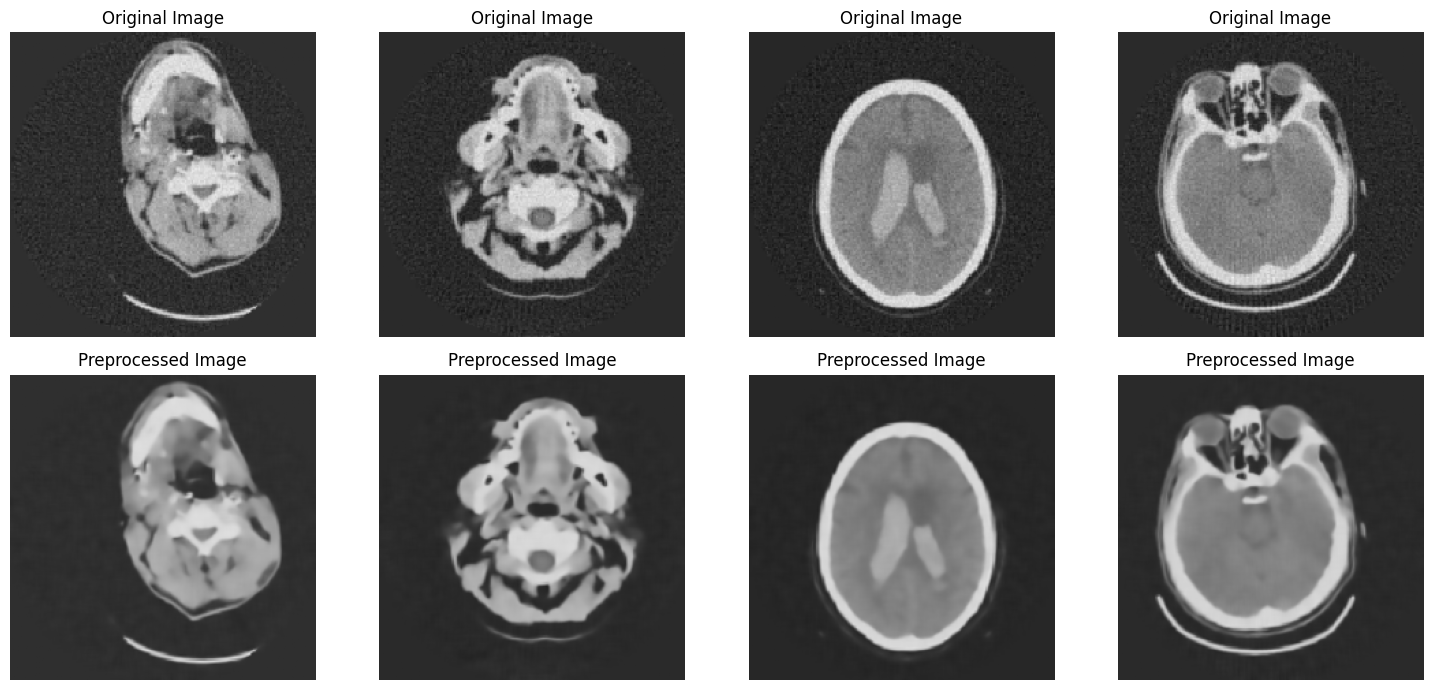
\includegraphics[width=0.75\textwidth]{denoiser.png}
    \caption{Test data sample before and after denoising layer} 
\end{figure}

\begin{par}
    Even though the scope of the project focused only on Gaussian and Poisson noises, we also implemented denoising functions for other common types of noise in CT scans to be used in future experiments:
    \begin{enumerate}
        \item Salt and pepper noise: we used a median filter on the image with a kernel size of 3x3. 3x3 was chosen because it was the right balance between blurring and keeping the important features of the image. 
        \item Speckle noise: To remove speckle noise, a bilateral filter was applied to the image as well as an estimation of the standard deviation of the color and spatial spaces. It was important to note that for all the functions, the multichannel was set to false as these were black and white CT images.
    \end{enumerate}
\end{par}

\newpage
\section{Results}

\begin{par}
A balanced subset extracted from the RSNA dataset consisting of 2000 control patients with no haemorrhage and 2000 patients with ICH was considered for this retrospective study. A physics informed machine learning model was developed and evaluated to study the effects of noise on CT images, A CNN model was tested without simulated noise and baseline performance was evaluated. To simulate low-dose CT imaging modality, Gaussian and Poisson noise was added to the physics informed machine learning model. 
\end{par}

\subsection{Gaussian Noise Experiment}
In Table 1 it is possible to see the results of the experiment with Gaussian noise. For each of the models trained on images with different levels of noise there is the accuracy result when making predictions on the test set with each level of noise added. It would be fair to assume that the model will always perform better on the test set with the same level of noise used during train, which is true for most cases, but there are some exceptions like 0 and 1.
The most important result and assumption we take from this experiment is that by applying a medium level of noise like 0.5 or 0.75 achieves the best overall accuracy when predicting ICH in CT scans with noise values between 0 and 1.5.

\vspace{0.5cm}
\begin{table}[h]
    \centering
    \caption{Gaussian Noise Evaluation Accuracy}
    \begin{tabular}{@{}llllllll@{}}
        \toprule
        Training Noise & Overall Acc & Test 0.0 & Test 0.25 & Test 0.5 & Test 0.75 & Test 1.0 & Test 1.5 \\
        \midrule
        0.0 & 67.64\% & 68.12\% & 68.25\% & 67.25\% & 68.62\% & 68.00\% & 65.62\% \\
        \midrule
        0.25 & 69.72\% & 69.83\% & 70.84\% & 68.67\% & 68.24\% & 69.55\% & 69.23\% \\
        \midrule
        0.5 & 73.96\% & 74.75\% & 74.75\% & 75.13\% & 74.50\% & 73.63\% & 71.00\% \\
        \midrule
        0.75 & 72.15\% & 70.13\% & 72.38\% & 73.88\% & 74.63\% & 71.88\% & 70.00\%\\
        \midrule
        1 & 67.79\% & 67.5\% & 67.88\% & 67.75\% & 68.00\% & 67.50\% & 68.13\% \\
        \midrule
        1.5 & 66.48\% & 65.95\% & 66.63\% & 66.38\% & 66.13\% & 66.25\% & 66.75\% \\
        \bottomrule
    \end{tabular}
\end{table}

\subsection{Poisson Noise Experiment}
\begin{par}
    The Poisson noise analysis was performed using Matlab/Python for a patient identification number ID04a0a875e diagnosed with ICH. Figure 5 shows sinogram heat maps simulating low light conditions (low photon count) due to CT scanner noise caused from detector inefficiency.The sinogram noise threshold for poison noise was increased from 1 to 5. The higher scaling factors lose the vital brain details that are necessary for making an accurate diagnosis.  
    In Table 2 are shown the overall results when training and testing the model with different levels of Poisson noise. 
\end{par}

\begin{table}[h]
    \centering
    \caption{Poisson Noise Evaluation Accuracy} 
    \begin{tabular}{@{}ll@{}}
        \toprule
        Training Noise & Accuracy \\
        \midrule
        0.0 & 62\% \\
        \midrule
        1 & 62.5\% \\
        \midrule
        2 & 41.6\% \\
        \midrule
        2.5 & 52\% \\
        \midrule
        3 & 48.6\% \\
        \midrule
        4 & 48.5\% \\
        \midrule
        5 & 52\% \\
        \bottomrule
    \end{tabular}
\end{table}

\begin{figure}[h]
  \centering
  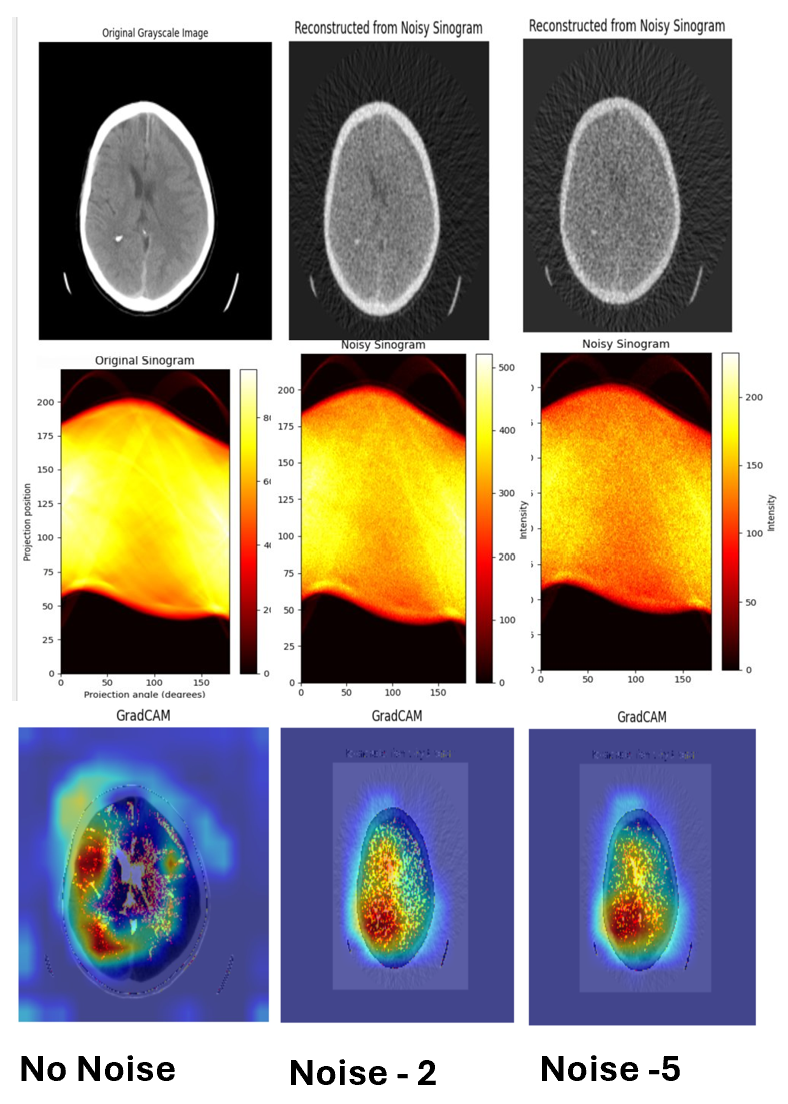
\includegraphics[width=0.5\textwidth]{sinogram_gradcam.png}
  \caption{Poisson Noise Sinogram Noise Threshold Heatmaps and associated Gradcam images}
\end{figure}

\section{Discussion }
\begin{par}
    In this retrospective study, we simulated real world  noise and evaluated the performance of our physics informed machine learning pipeline.
    To develop an accurate and precise denoising algorithm that can reconstruct finer details of CT images it is paramount to know the effects of real world noise on CT images. Therefore this study informs us of the optimal noise threshold required to preserve clinical details of CT images. Gaussian sinogram noise simulates real world CT noise like sensor noise, thermal noise (Johnson-Nyquist noise), shot noise caused by the discrete nature of electric charge, and background radiation noise from natural sources like the sun and the earth. Poisson sinogram noise also called as photon counting noise is related to image intensity and changing noise threshold using a scaling factor effectively changes the photon counts. The pixel values are proportional to the photons detected [2]. Due to the absence of fixed variance like the Gaussian noise, changes in Poisson noise can be used to simulate real world CT scanner noise due to detector inefficiency or low photon count.
\end{par}

\section{Limitations and Future Work} 
\begin{par}
    One of the major limitations of this study is that only a subset of the RSNA dataset was evaluated due to computational limitations. Since we performed full-training of a VGG16 model it would have needed a bigger dataset during training to learn the particular characteristics of medical imaging (especially CT Scans).
    Despite those limitations, Gaussian noise analysis results show that the training noise threshold of 0.5 and 0.75 showed superior performance than the baseline. Poisson noise experiments helped us understand the various issues that are caused due to the randomness in photon detection. Applying data augmentations and hyperparameter tuning to the model showed improvement than the baseline. The higher noise thresholds did not lead to good reconstruction of sinogram. GradCam analysis was performed to understand the noise distribution during deep learning. Higher noise threshold greater than 1.5 showed that our model could not detect the finer details of the CT image. 
    Future work for this study may involve two major improvements:
    \begin{enumerate}
        \item Physical transformations: improve the noising/denoising techniques to be more realistic, and test other types of noise and combinations of noise types in the same test set. Fine-tune the sinogram reconstruction process to make the process more efficient and less information lossy.
        \item Modeling: to achieve higher validation/testing performance and be able to analyse more precise changes in accuracy of the different noise levels we can fine-tune a pretrained model that was already fine-tuned on medical data such as "TencentMedicalNet/MedicalNet-Resnet10" publicly available on HuggingFace. Since this model is capable of analysing medical image out-of-the-box, it is expected that the subset we used for this study is enough for the model to learn the specific patterns of ICH detection.
    \end{enumerate}
\end{par}

%%%%%%%%%%%%%%%%%%%%%%%%%%%%%%%%%%%%%%%
%Bibliography

\begin{thebibliography}{99}

\bibitem{Lecun15} 
Goldman LW. Principles of CT and CT technology. J Nucl Med Technol. 2007 Sep;35(3):115-28; quiz 129-30. doi: 10.2967/jnmt.107.042978. PMID: 17823453.
\bibitem{Lecun15} 
Manoj Diwakar, Manoj Kumar. A review on CT image noise and its denoising,
Biomedical Signal Processing and Control,Volume 42, 2018, Pages 73-88,
ISSN 1746-8094.
\bibitem{Lecun15}
Caceres JA, Goldstein JN. Intracranial hemorrhage. Emerg Med Clin North Am. 2012 Aug;30(3):771-94. doi: 10.1016/j.emc.2012.06.003. PMID: 22974648; PMCID: PMC3443867.
\bibitem{Lecun15}
Broderick J, Connolly S, Feldmann E, Hanley D, Kase C, Krieger D, Mayberg M, Morgenstern L, Ogilvy CS, Vespa P, Zuccarello M; Guidelines for the management of spontaneous intracerebral hemorrhage in adults: 2007 update: a guideline from the American Heart Association/American Stroke Association Stroke Council, High Blood Pressure Research Council, and the Quality of Care and Outcomes in Research Interdisciplinary Working Group. Circulation. 2007 Oct 16;116(16):e391-413. doi: 10.1161/CIRCULATIONAHA.107.183689. PMID: 17938297.
\bibitem{Lecun15}
Lee JY, Kim JS, Kim TY, Kim YS. Detection and classification of intracranial haemorrhage on CT images using a novel deep-learning algorithm. Sci Rep. 2020 Nov 25;10(1):20546. doi: 10.1038/s41598-020-77441-z. PMID: 33239711; PMCID: PMC7689498.
\bibitem{Lecun15}
Yang S, Pu Q, Lei C, Zhang Q, Jeon S, Yang X. Low-dose CT denoising with a high-level feature refinement and dynamic convolution network. Med Phys. 2023 Jun;50(6):3597-3611. doi: 10.1002/mp.16175. Epub 2023 Jan 7. PMID: 36542402.
\bibitem{Lecun15}
Lierová A, Milanová M, Pospíchal J, Novotný J, Storm J, Andrejsová L, Šinkorová Z. BIOLOGICAL EFFECTS OF LOW-DOSE RADIATION FROM CT IMAGING. Radiat Prot Dosimetry. 2022 Aug 22;198(9-11):514-520. doi: 10.1093/rpd/ncac091. PMID: 36005951.
\bibitem{Lecun15}
Solomon JB, Li X, Samei E. Relating noise to image quality indicators in CT examinations with tube current modulation. AJR Am J Roentgenol. 2013 Mar;200(3):592-600. doi: 10.2214/AJR.12.8580. PMID: 23436849.
\bibitem{Lecun15}
Li, T., Li, X., Wang, J., Wen, J., Lu, H., Hsieh, J., & Liang, Z. (2004). Nonlinear sinogram smoothing for low-dose X-ray CT. IEEE Transactions on Nuclear Science, 51(5 II), 2505-2513. https://doi.org/10.1109/TNS.2004.834824
\bibitem{Lecun15}
Borsdorf A, Raupach R, Flohr T, Hornegger J. Wavelet based noise reduction in CT-images using correlation analysis. IEEE Trans Med Imaging. 2008 Dec;27(12):1685-703. doi: 10.1109/TMI.2008.923983. PMID: 19033085.
\bibitem{Lecun15}
Bhadauria HS, Dewal ML. Efficient denoising technique for CT images to enhance brain hemorrhage segmentation. J Digit Imaging. 2012 Dec;25(6):782-91. doi: 10.1007/s10278-012-9453-y. PMID: 22274942; PMCID: PMC3491154.
\bibitem{Lecun15}
C Anam, T Fujibuchi, T Toyoda, N Sato, F Haryanto, R Widita, I Arif and G Dougherty. An investigation of a CT noise reduction using a modified of wiener filtering-edge detection, Journal of Physics, 2019
\bibitem{Lecun15}
Korbinian Mechlem, Sebastian Allner, Kai Mei, Franz Pfeiffer, Peter B. Noël, "Dictionary-based image denoising for dual energy computed tomography," Proc. SPIE 9783, Medical Imaging 2016: Physics of Medical Imaging, 97830E (22 March 2016)
\bibitem{Lecun15}
Sadia RT, Chen J, Zhang J. CT image denoising methods for image quality improvement and radiation dose reduction. J Appl Clin Med Phys. 2024 Feb;25(2):e14270. doi: 10.1002/acm2.14270. Epub 2024 Jan 19. PMID: 38240466; PMCID: PMC10860577.
\bibitem{Lecun15}
Li M, Hsu W, Xie X, Cong J, Gao W. SACNN: Self-Attention Convolutional Neural Network for Low-Dose CT Denoising With Self-Supervised Perceptual Loss Network. IEEE Trans Med Imaging. 2020 Jul;39(7):2289-2301. doi: 10.1109/TMI.2020.2968472. Epub 2020 Jan 21. PMID: 31985412
\bibitem{Lecun15}
Wang W, Gang GJ, Stayman JW. A CT Denoising Neural Network with Image Properties Parameterization and Control. Proc SPIE Int Soc Opt Eng. 2021 Feb;11595:115950K. doi: 10.1117/12.2582145. Epub 2021 Feb 15. PMID: 34646056; PMCID: PMC8506264.
\bibitem{Lecun15}
Yi X, Babyn P. Sharpness-Aware Low-Dose CT Denoising Using Conditional Generative Adversarial Network. J Digit Imaging. 2018 Oct;31(5):655-669. doi: 10.1007/s10278-018-0056-0. PMID: 29464432; PMCID: PMC6148809.
\bibitem{Lecun15}
Wang G, Hu X. Low-dose CT denoising using a Progressive Wasserstein generative adversarial network. Comput Biol Med. 2021 Aug;135:104625. doi: 10.1016/j.compbiomed.2021.104625. Epub 2021 Jul 3. PMID: 34246157.
\bibitem{Lecun15}
H. Li, X. Yang, S. Yang, D. Wang and G. Jeon, "Transformer With Double Enhancement for Low-Dose CT Denoising," in IEEE Journal of Biomedical and Health Informatics, vol. 27, no. 10, pp. 4660-4671, Oct. 2023, doi: 10.1109/JBHI.2022.3216887
\bibitem{Lecun15}
Ju Zhang, Zhibo Shangguan, Weiwei Gong, Yun Cheng, A novel denoising method for low-dose CT images based on transformer and CNN, Computers in Biology and Medicine, Volume 163, 2023, 107162, ISSN 0010-4825
\bibitem{Lecun15}
Flanders AE, Prevedello LM, Shih G, Halabi SS, Kalpathy-Cramer J, Ball R, Mongan JT, Stein A, Kitamura FC, Lungren MP, Choudhary G, Cala L, Coelho L, Mogensen M, Morón F, Miller E, Ikuta I, Zohrabian V, McDonnell O, Lincoln C, Shah L, Joyner D, Agarwal A, Lee RK, Nath J; RSNA-ASNR 2019 Brain Hemorrhage CT Annotators. Construction of a Machine Learning Dataset through Collaboration: The RSNA 2019 Brain CT Hemorrhage Challenge. Radiol Artif Intell. 2020 Apr 29;2(3):e190211. doi: 10.1148/ryai.2020190211. Erratum in: Radiol Artif Intell. 2020 Jul 29;2(4):e209002. PMID: 33937827; PMCID: PMC8082297.

 \end{thebibliography}

\end{document}